\section{Comparison between the ridge and Lasso estimators} \label{sec:5.CRL}
We now have all the necessary tools to compare ridge regression with the Lasso. We do so with an elaborate example in R. The data set used in the rest of this section was found on \textit{Kaggle.com} \cite{EpiR}.

\subsection{The data}
The data set we will be using is about recipes from a popular website. It contains \num{20 025} observations (i.e. recipes) of \num{680} variables. Most of these variables are binary, indicating categories such as \textit{contains cucumber} or \textit{is a 22-minute meal}. Each recipe also has a \textit{rating}: a value that measures how well liked the recipe is by the users of the website.

In what follows, we will try to analyze the effect of all these variables on the rating of the recipes with regular least squares regression, ridge regression and the Lasso. We will compare their prediction accuracy and, along the way, illustrate some properties of the ridge and Lasso estimator. Lastly, we use the Lasso the find out which ingredients we should use and which styles of cooking we should follow in order to get the statistically most liked recipe.

Before we can begin, we must first remove all observations in the data set that contain values \textit{NA} as the built-in methods from the \textit{GLMNET}-package fail when these values are present. We also rename some badly named columns, remove the column containing the names of the recipes as this is not a predictor and restrict the data set to its first \num{15 000} observations. This last modification is done in order to work with nicely rounded numbers, which will be useful when dividing the observations into training and test sets, as well as reducing computation time. All of these modifications leave us with a data set containing 15 000 observations of 679 variables.

To illustrate the advantage of ridge and Lasso over regular least squares regression when $n \approx p$ we also simulate a small data set containing 120 observations of 51 variables (this way we have 50 predictors for the variable \textit{rating}). The reason why we simulate this data instead of just restricting the existing data set is that the latter leads to linearly dependent columns, so that we cannot apply linear regression.

\subsection{Regular least squares regression}
When we try to apply linear regression on the data set, the method fails. This failure is probably due to some columns of the data matrix being linearly dependent. Therefore other methods like ridge regression or the Lasso should be used. We also apply linear regression on the simulated data set. Since $n \approx p$, the MSE is very high, attaining a value of \num{24.3630}. This number means that, on average, the score we predict will be wrong by about $\sqrt{24.3630} \approx 5$ points. Since the scores is a number between $0$ and $5$, we get (almost) no valuable information from this model.

\subsection{Subset selection using the Lasso} \label{sec:SubsetSelectionUsingLasso}
Next we apply the Lasso to the data set and see which predictors it selects as the 10 most important. We get the following result:
\begin{center}
\begin{tabular}{ccc}
    \vspace{3pt}
     "caviar" & "cuba" & "dorie greenspan"\\
     \vspace{3pt}
     "germany" & "kitchen olympics" & "pancake"\\
     \vspace{3pt}
     "philippines" & "sardine" & "sorbet"\\
     & "leftovers" &
\end{tabular}
\end{center}
Note that these categories can either indicate a very high or very low rating.\\
\\
In order to test that the Lasso indeed indicates which predictors are the most important, we can artificially modify one predictor of the data set to be a 'perfect predictor' of the rating. In this example, we take the predictor \textit{22-minute meal} and set it to 1 if the rating of the recipe is bigger then 3. Therefore, the value of \textit{22-minute meal} should give a very good indication of the rating of the recipe and as a consequence, the Lasso should give it a high regression coefficient. Implementing the above into R and applying the Lasso, we get:
\begin{center}
    \begin{tabular}{ccc}
    \vspace{3pt}
        "22-minute meals" & "3-ingredient recipes" & "biscuit"\\
        \vspace{3pt}
        "flaming hot summer" & "gin" & "house \& garden"\\
        \vspace{3pt}
        "idaho" & "kansas" & "pastry"\\
        & "leftovers" &
    \end{tabular}
\end{center}
As expected, the Lasso now selects the predictor \textit{22-minute meal} as one of the 10 most important predictors.

Before continuing to the next section, we undo our changes to the variable \textit{22-minute meal}.

\subsection{Applying ridge regression} \label{sec:ApplyingRidgeRegression}
In this section we apply ridge regression on the data set. In order to properly asses the test error of the ridge model, we should carry out 10-fold Cross-Validation as explained in section~\ref{sec:4.CV&PS}. However, this would take hours of computing time. In order to have code that we -- or you, the reader -- can modify easily to explore the problem further without having to wait hours for the computations to complete each time, we opt to use training sets of size \num{10 000} and hence only have to compute the ridge model three times (even this already takes up a couple of minutes). Doing so gives us a test error of \num{1.5468}. Applying ridge regression on the simulated data set, we get a test error of \num{1.4888}. This is a tremendous improvement on the test error we got from the regular least squares model.

Like in Section~\ref{sec:PractRidgeComparison} we plot the size of the regression coefficients in function of $\lambda$ in Figure~\ref{fig:CoeffRidgeExample}. As this is only a general illustration of how the coefficients tend to evolve in function of $\lambda$, we part with Cross-Validation all together and just use a fixed training and test set. Figure~\ref{fig:CoeffRidgeExample} illustrates nicely how all coefficients get shrunk towards zero.

\begin{figure}
    \centering
    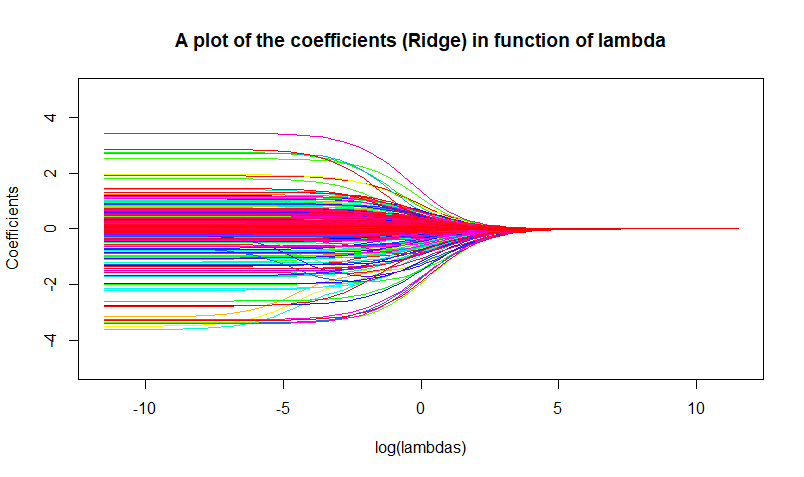
\includegraphics[width=\linewidth]{Figures/Coeff_Lambda_plot_ridge.png}
    \caption{The coefficients of the ridge model in function of $\lambda$.}
    \label{fig:CoeffRidgeExample}
\end{figure}

\subsection{Applying the Lasso} \label{sec:ApplyingTheLasso}
We continue our analysis by applying the Lasso on the data set. For similar reasons as in Section~\ref{sec:ApplyingRidgeRegression} we use training sets of size \num{10 000} and thus compute the Lasso model only thrice. The resulting test error of the model is \num{1.1790}. This is better than that of the ridge model. Applying the Lasso on the simulated data set, we get a test error of \num{1.4879}. This is also better than the one we got using ridge regression, although only very slightly. A plot of the coefficients of the Lasso model is given in Figure~\ref{fig:CoeffLassoExample}.

\begin{figure}
    \centering
    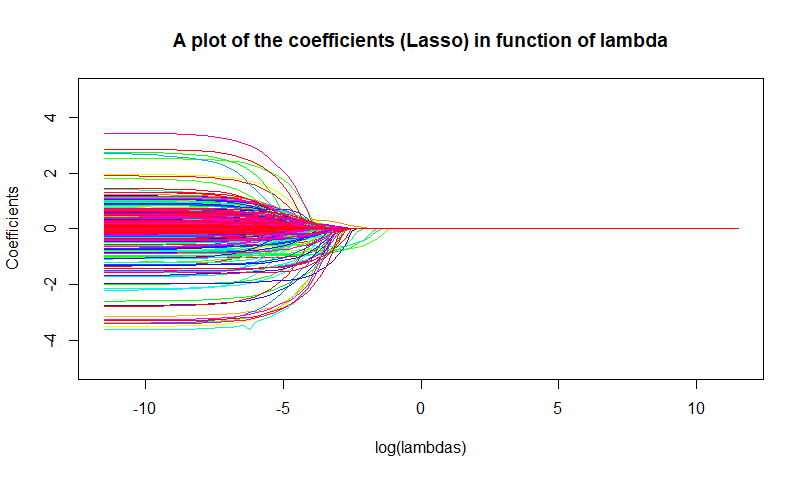
\includegraphics[width=\linewidth]{Figures/Coeff_Lambda_plot_Lasso.png}
    \caption{The coefficients of the Lasso model in function of $\lambda$.}
    \label{fig:CoeffLassoExample}
\end{figure}

Figure~\ref{fig:Comparison_ridge_Lasso} compares, for fixed training and test set, the MSE of the ridge and Lasso model.\footnote{Hence we again do not implement any form of Cross-Validation for this figure. this is why the mean squared errors for the optimal values of lambda slightly differ from the mean squared errors we got in Section~\ref{sec:ApplyingRidgeRegression} and~\ref{sec:ApplyingTheLasso}.} The plot shows an important difference in characteristic of ridge and Lasso estimation: The curve of the mean squared error appears smooth for ridge regression, but shows a discontinuity in the first derivative in the case of the Lasso. This difference can be explained by the 'subset-selection property' of the latter estimator. When regression coefficients for the Lasso model get small enough, they get set exactly equal to zero and remain zero, in contrast to ridge regression, where they \textit{approach} zero and can oscillate around zero. A similar difference in behaviour can also be seen from Figures~\ref{fig:CoeffRidge} and~\ref{fig:CoeffLasso}.

\begin{figure}
    \centering
    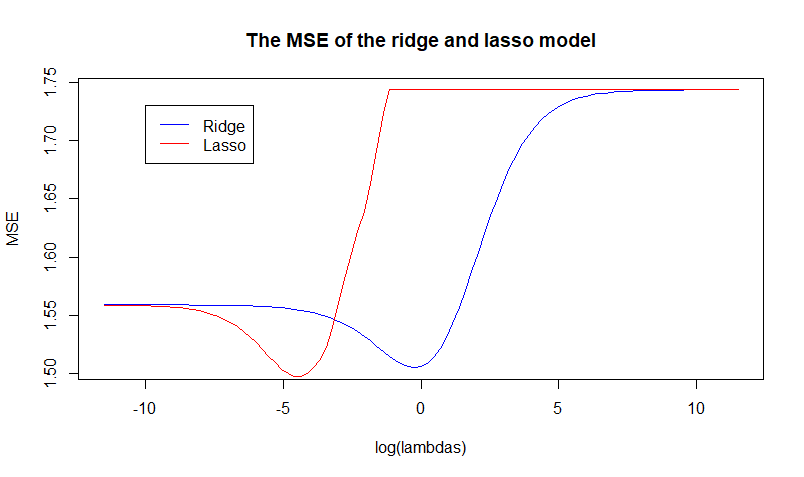
\includegraphics[width=\linewidth]{Figures/Comparison_ridge_lasso.png}
    \caption{A plot comparing the MSE of the ridge and lasso model in function of $\lambda$. The models were computed with the same training data and the test errors were calculated with the same test data.}
    \label{fig:Comparison_ridge_Lasso}
\end{figure}

\subsection{Some data analysis using the Lasso}
To conclude this section, we perform some data analysis using the Lasso. More specifically, we try to answer the following two questions:
\begin{itemize}
    \item Which nutritional values \textit{calories}, \textit{fat}, \textit{protein} and \textit{sodium} should a recipe have to get the highest rating?
    \item What categories should a recipe belong to (or definitely not belong to) in order to have the highest rating?
\end{itemize}
To answer the first question, we restrict our data to just the 5 columns \textit{rating}, \textit{calories}, \textit{fat}, \textit{protein} and \textit{sodium} and apply the Lasso. We get the following output, listed in Table~\ref{tab:NutritionalValues}.
\begin{table}[h]
    \centering
    \begin{tabular}{cc}
         calories & \num{2.258779e-08}\\
         protein & \num{5.776022e-06}\\
         fat & \num{-7.529660e-07}\\
         sodium & .
    \end{tabular}
    \caption{Analysis of the nutritional values}
    \label{tab:NutritionalValues}
\end{table}
From the regression coefficients we can see that recipes with high protein tend to get given a high rating, and that the amount of fat in a recipe has a negative impact on the rating. In other words: If we want a recipe with high rating, we should cook healthy!\\
\\
To answer the second question we perform the Lasso on the data set where the columns containing nutritional value (\textit{calories}, \textit{fat}, \textit{protein} and \textit{sodium}) have been removed. Similar to Section~\ref{sec:SubsetSelectionUsingLasso} we select the \num{10} predictors that have the highest coefficients in absolute value. This time we also note down their numerical values. The results are listed in Table~\ref{tab:Ingredients}.
\begin{table}[h]
    \centering
    \begin{tabular}{c|c}
        leftovers &  -3.45301190707604 \\
        kitchen olympics &  -2.68671340475449 \\
        germany &  -2.68045838198475 \\
        sardine &  -2.49597552609873 \\
        dorie greenspan &  -2.38525177319951 \\
        caviar &  -2.24005956660075 \\
        cuba &  -2.11104676712887 \\
        philippines &  -2.09261833766479 \\
        pancake &  -2.04455056659949 \\
        sorbet &  -1.87835922993761 \\
    \end{tabular}
    \caption{Analysis of the different categories}
    \label{tab:Ingredients}
\end{table}
All of the categories above have a negative regression coefficient. This means we should definitely avoid designing a recipe that belongs to any of them. 